% IEEE-style technical report: geometric deep learning surrogates for 2D bluff-body CFD.
% Build from this directory:  pdflatex main && pdflatex main
% Figures are referenced from the repository root through \graphicspath.
\documentclass[journal]{IEEEtran}

\usepackage[T1]{fontenc}
\usepackage{amsmath,amssymb,amsfonts}
\usepackage{graphicx}
\usepackage{booktabs}
\usepackage{multirow}
\usepackage{array}
\usepackage{xcolor}
\usepackage{url}
\usepackage{cite}
\usepackage{tikz}
\usetikzlibrary{positioning,arrows.meta,fit}
\usepackage[hidelinks]{hyperref}

\graphicspath{{../}}
\newcommand{\Cp}{C_p}
\newcommand{\RMSE}{\mathrm{RMSE}}
\newcommand{\nb}{\mathrm{nb}}
\newcommand{\pdone}{P_{D1,r}}
\newcommand{\pdtwo}{P_{D2,r}}
\newcommand{\Vin}{V_{\infty}}
\newcommand{\hyp}[1]{\textit{Hypothesis:} #1}

\begin{document}

\title{Mesh-Based Geometric Deep Learning Surrogates for Parametric Bluff-Body Flow:\\
Physical Target Scaling, Near-Body Loss Balancing, and Global Attention}

\author{Geometric Deep Learning CFD Project
\thanks{Technical report compiled on 20 November 2026 from the project repository,
its research diary (\texttt{RESEARCH\_LOG.md}) and all saved experiment artifacts.
All numbers are taken from saved JSON reports; analyses performed while
preparing this report are labelled as such.}}

\markboth{Technical Report, November 2026}{Geometric Deep Learning Surrogates for Bluff-Body CFD}

\maketitle

\begin{abstract}
We report a complete account of a research programme that builds graph neural
network (GNN) reduced-order models (ROMs) of the steady pressure field around a
parametric two-dimensional bluff body simulated with STAR-CCM+.
The dataset contains 30 designs spanned by two shape parameters and the inlet
speed, totalling 279{,}177 fluid cells and 1{,}415{,}224 directed adjacency edges.
We construct cell-centred graphs directly from the finite-volume export,
reconstruct cell areas from closed face loops, and study, in sequence:
(i) dynamic-pressure (pressure-coefficient) target scaling and dimensionless
geometric features under five-fold cross-validation;
(ii) single-design reconstruction capacity;
(iii) a near-body-balanced, area-normalised loss;
(iv) two forms of attention --- edge-aware neighbour attention and a latent-token
global attention block that approximates all-to-all communication at
$\mathcal{O}(NM+M^2)$ cost;
(v) parameter-matched controls; and
(vi) the effect of replacing ReLU/GELU/LeakyReLU nonlinearities with $\tanh$.
Coefficient targets reduced mean per-design RMSE by 13.8\,\% in five-fold
cross-validation. On one fixed outer fold, the near-body loss halved near-body
RMSE (29.60$\rightarrow$14.70\,Pa) at a cost of 8.1\,\% whole-domain RMSE.
In a nested protocol with inner-validation checkpoint selection, a width-32 GNN
with 32 latent tokens and $\tanh$ activations achieved the best observed mean
whole-domain RMSE (2.92\,Pa), near-body RMSE (9.35\,Pa) and worst-design RMSE
(3.97\,Pa), against 4.97, 19.93 and 6.72\,Pa for the original width-32 GNN.
A parameter-matched plain GNN recovered most of the gap in whole-domain error,
showing that capacity is a large part of the effect.
We emphasise that all architecture comparisons use one seed and one outer fold
whose six designs had been inspected earlier; they are exploratory, not an
unbiased test. A retrospective analysis performed for this report further shows
that the inner-training set contains no design with $\pdone<0.114$, whereas the
two hardest outer designs and three of five inner-validation designs lie at
$\pdone\approx0.05$; the hardest cases are therefore parametric extrapolations.
We document negative results, compromises, and a concrete plan to obtain
unbiased conclusions.
\end{abstract}

\begin{IEEEkeywords}
Geometric deep learning, graph neural networks, reduced-order modelling,
computational fluid dynamics, attention, surrogate modelling, nested cross-validation.
\end{IEEEkeywords}

% =============================================================================
\section{Introduction}
% =============================================================================
\IEEEPARstart{D}{esign} exploration with high-fidelity computational fluid dynamics
(CFD) is limited by solver cost. Machine-learned reduced-order models (ROMs)
promise near-instant field predictions for new designs, but they must generalise
across geometry changes, unstructured meshes of varying size, and flow regimes,
while remaining accurate where it matters most physically: close to the body,
where pressure gradients are steep and the integrated loads are determined.

Mesh-based graph neural networks~\cite{battaglia2018,gilmer2017,pfaff2021}
operate natively on unstructured finite-volume meshes and are therefore an
attractive choice. Their main weakness is locality: $L$ message-passing layers
propagate information only $L$ graph hops, while pressure in incompressible flow
is governed by an elliptic constraint with global influence. Transformer-style
neural operators~\cite{vaswani2017,hao2023gnot,wu2024transolver} offer global
communication but full self-attention scales quadratically with the number of
cells. The commercial reference workflow that motivated this study (Siemens
STAR-CCM+ PhysicsAI~\cite{siemens_train,siemens_validate,siemens_ref,siemens_theory})
uses transformer-based operator learning.

This report documents, end to end, a series of experiments on a 30-design
two-dimensional bluff-body dataset. It is written as a research record rather
than a success story: every change is motivated, measured under an explicit
protocol, inspected visually, and its limitations stated. Contributions are:
\begin{enumerate}
\item A verified pipeline that converts STAR-CCM+ \texttt{.simh} (HDF5) volume
exports into cell graphs, reconstructing cell areas from face loops with
$\approx\!6\times10^{-8}$ relative agreement to an independent calculation
(Section~\ref{sec:data}).
\item A five-fold cross-validated study of physical target scaling and
dimensionless geometric features (Section~\ref{sec:exp_cv}).
\item A diagnosis separating representation capacity from generalisation, and a
near-body-balanced loss that corrects a severe area-weighting imbalance:
the region within 0.05\,m of the wall contains 67.6\,\% of cells but only
1.73\,\% of the fluid area (Sections~\ref{sec:exp_overfit}--\ref{sec:exp_loss}).
\item A graph-isolated latent-token global attention block and an edge-aware
neighbour attention aggregator, both optional and backward compatible
(Section~\ref{sec:models}).
\item A nested model-selection protocol, parameter-matched controls, an explicit
multi-criterion ranking, and an activation study (Sections~\ref{sec:exp_nested}--\ref{sec:exp_tanh}).
\item A critical analysis of confounds --- capacity, learning-rate schedule,
validation noise, fold reuse and parametric extrapolation --- with a plan to
remove them (Sections~\ref{sec:discussion}--\ref{sec:future}).
\end{enumerate}

% =============================================================================
\section{Related Work}
% =============================================================================
\textbf{Graph networks for simulation.}
Message-passing neural networks~\cite{gilmer2017} and the graph-network
framework~\cite{battaglia2018} underlie mesh-based simulators such as
MeshGraphNets~\cite{pfaff2021}, which use an encode--process--decode structure; our base model follows this design with an edge-message MLP and a residual node-update MLP.
Geodesic convolutional networks were used early on for shape-dependent
aerodynamic prediction~\cite{baque2018}, and convolutional U-Nets on
interpolated grids for airfoil flow fields~\cite{thuerey2020}.

\textbf{Attention.} Graph attention~\cite{velickovic2018} and its more
expressive GATv2 variant~\cite{brody2022} replace fixed aggregation by learned
neighbour weights. Our neighbour attention computes scores from both endpoint
states and edge features, similar in spirit to GATv2, but uses the learned edge
message as the value. To obtain global communication without quadratic cost,
we use a learned latent bottleneck as in the Set Transformer's induced
attention~\cite{lee2019set} and Perceiver~\cite{jaegle2021perceiver}; physics
transformers such as GNOT~\cite{hao2023gnot} and Transolver~\cite{wu2024transolver}
use related linear-cost mechanisms. Fourier neural operators~\cite{li2021fno}
are an alternative that require regular grids or a mapping to one.

\textbf{Physics-informed training.} Physics-informed networks~\cite{raissi2019}
add PDE residuals; we use the weaker but robust option of physically scaled
targets and a differentiable integrated-load loss for the surface model.

\textbf{Evaluation methodology.} Selecting hyperparameters on the same data
used to report performance biases error estimates optimistically~\cite{varma2006,cawley2010};
this motivates our nested protocol and our caution about reusing an inspected fold.

% =============================================================================
\section{Problem Definition and Data}
\label{sec:data}
% =============================================================================
\subsection{Physical Problem}
The flow is steady, incompressible and planar, around a single body centred
near $(0.5, 0.5)$\,m in a rectangular domain $x\in[0,3]$\,m,
$y\in[0,1]$\,m (fluid area $\approx2.94$\,m$^2$ per design).
Each design is defined by
$\boldsymbol{\theta}=(\pdone,\pdtwo,\Vin)$: two CAD shape parameters and the
inlet speed. Figure~\ref{fig:eda} shows the resulting family of shapes,
ranging from a very small, nearly square body ($\pdone\approx0.05$) to large
diamond- and kite-shaped bodies.
Density is $\rho=1.18415$\,kg\,m$^{-3}$ and outlet gauge pressure is
0\,Pa in every design (verified across all 30 exports).

\begin{figure}[!t]
\centering
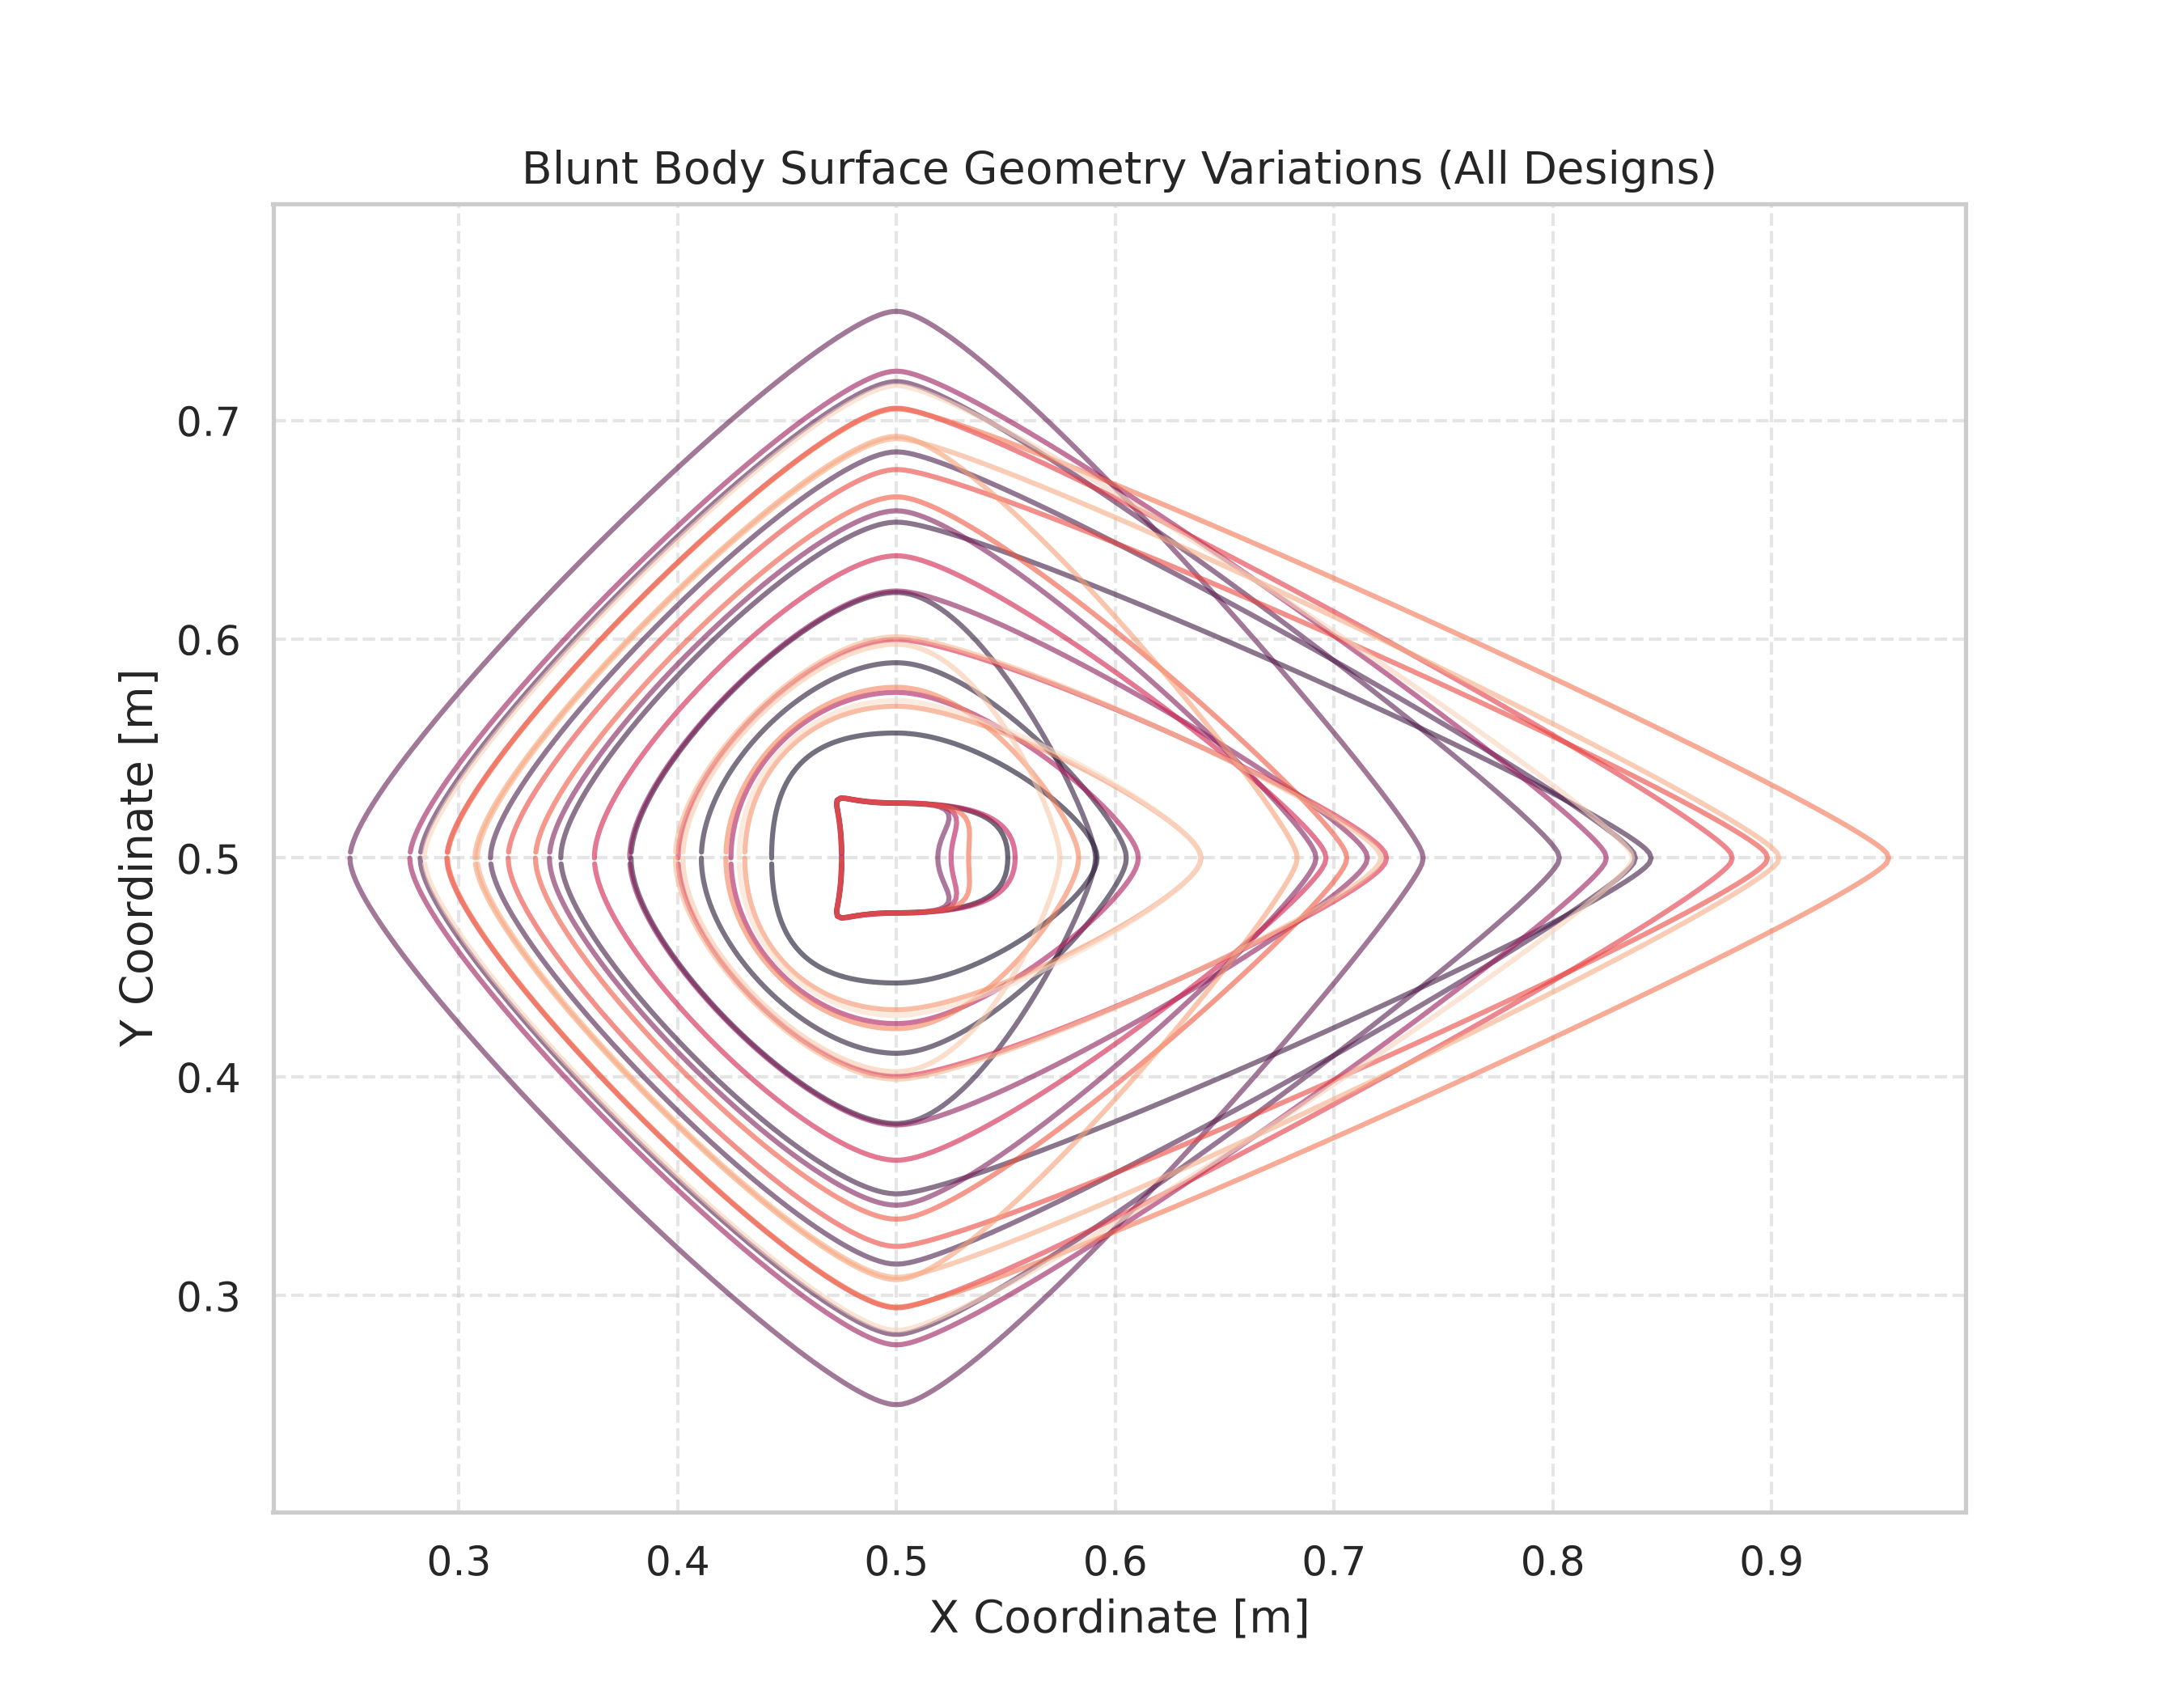
\includegraphics[width=\columnwidth]{EDA_Results/3_geometric_shape_variations.png}
\caption{Body outlines of all 30 designs, extracted from the surface exports.
The small near-square shapes correspond to $\pdone\approx0.05$.}
\label{fig:eda}
\end{figure}

\subsection{Dataset}
The data comprise 30 STAR-CCM+ designs in a folder named
\emph{Training\_Adaptive\_Sampling}. Design parameters lie in
$\pdone\in[0.05,0.5]$, $\pdtwo\in[0.75,2.25]$ and $\Vin\in[7.5,12.5]$\,m/s.
(The first eight designs follow a regular stratified pattern in $\pdone$,
Design\_9 is the all-minimum corner, and Designs\_10--30 appear to come from
adaptive sampling; this is inferred from the parameter values, not documented.)
Reported drag ranges from 2.04\,N (Design\_2) to 121.17\,N (Design\_7), a
59-fold span. Table~\ref{tab:data} summarises the meshes.

\begin{table}[!t]
\centering
\caption{Dataset Statistics (All 30 Designs)}
\label{tab:data}
\begin{tabular}{lr}
\toprule
Quantity & Value \\
\midrule
Designs & 30 \\
Fluid cells, total & 279{,}177 \\
Cells per design, min / mean / max & 3{,}958 / 9{,}306 / 15{,}243 \\
Directed cell-adjacency edges & 1{,}415{,}224 \\
Wall (surface) faces per design & 76 -- 590 \\
Cell pressure range & $-355.7$ to $262.8$\,Pa \\
Drag range (STAR-CCM+ report) & 2.04 -- 121.17\,N \\
Cells with wall distance $\le0.05$\,m & 67.6\,\% \\
Fluid area with wall distance $\le0.05$\,m & 1.73\,\% \\
\bottomrule
\end{tabular}
\end{table}

The last two rows, computed while preparing this report, quantify the mesh
refinement near the wall and are central to Section~\ref{sec:exp_loss}: any
area-weighted objective assigns under 2\,\% of its weight to the region that
determines surface loads.

\subsection{Scalar Reports}
Each design log provides the parameters and STAR-CCM+ reports for drag, drag
coefficient and pressure drop. The PressureDrop report is a scalar response,
not a field error. The reported $C_d$ is consistent with $C_d=F_D/(q_\infty
A_\mathrm{ref})$ using $A_\mathrm{ref}=0.005$\,m$^2$ and
$q_\infty=\tfrac12\rho\Vin^2$, which we confirmed numerically for Design\_1.

\subsection{Comparison with the Reference Workflow}
\label{sec:siemens}
The documented PhysicsAI tutorial~\cite{siemens_train,siemens_validate,siemens_ref,siemens_theory}
differs from our protocol in ways that make numerical comparison invalid:
it uses transformer-based operator learning with multi-head
self-attention~\cite{siemens_theory}; trains for 1{,}000 epochs with 300
field-model spatial sample points; uses a default 80/20 internal
training/validation split with selectable best-validation, best-training or
last checkpoint; and tests on 16 \emph{new} Latin-hypercube designs in a
narrower domain ($\pdone\in[0.1,0.2]$, $\pdtwo\in[1.5,2.0]$,
$\Vin\in[8,10]$\,m/s). Its PressureDrop accuracy comes from a separate scalar
response model. Our experiments therefore do not reproduce PhysicsAI and are
not directly comparable to its published tables.

% =============================================================================
\section{Graph Construction and Features}
\label{sec:graph}
% =============================================================================
\subsection{Volume Cell Graph}
The volume mesh is read from \texttt{Meshes/FvMesh~1/Regions/Domain}. We verify
that all vertex $z$-coordinates are equal (planar mesh) and that every face has
exactly two vertices. Each interior face with owner--neighbour cells $(i,j)$
contributes directed edges $i\!\to\!j$ and $j\!\to\!i$. Boundary faces are not
graph edges but are used to close cell polygons.

\textbf{Cell area reconstruction.} The export provides cell centroids but not
areas. For each cell we gather its interior and boundary faces, build a vertex
adjacency map, require every vertex to have exactly two incident faces, walk the
loop to obtain an ordered polygon (rejecting self-intersections and disconnected
loops), and apply the shoelace formula
\begin{equation}
A_i=\tfrac12\Big|\textstyle\sum_k x_k y_{k+1}-y_k x_{k+1}\Big|.
\end{equation}
Areas agree with an independent face-triangle calculation to
$\approx6\times10^{-8}$ relative error. The same polygons are used for plotting,
so visualisations show true cells rather than scattered centroids.

\textbf{Node features.} $\mathbf{g}_i=(x_i,y_i,z_i,A_i)$ for the baseline and
coefficient variants, and additionally the wall distance $d_i$ exported by
STAR-CCM+ for the geometry variant. The constant $z$ channel is harmless:
the standardiser replaces any standard deviation below $10^{-6}$ by one.
Design parameters $\boldsymbol{\theta}$ are broadcast to every node.

\textbf{Edge features (geometry variant).} For an edge $i\!\to\!j$ with
displacement $\Delta=\mathbf{x}_j-\mathbf{x}_i$ and local length scale
$\ell_{ij}=\sqrt{(A_i+A_j)/2}$,
\begin{equation}
\mathbf{e}_{ij}=\Big[\tfrac{\Delta}{\|\Delta\|},\;
\tfrac{\|\Delta\|}{\ell_{ij}},\;\log\tfrac{A_j}{A_i}\Big]\in\mathbb{R}^4.
\end{equation}
All four quantities are dimensionless and invariant to uniform mesh scaling;
the log-area ratio exposes grading in the refined near-wall mesh.

\subsection{Surface Face Graph}
For the earlier surface model, wall faces (two-vertex segments) are nodes with
features $(\mathbf{c},\mathbf{n},A)\in\mathbb{R}^7$ (centroid, normal, length).
Two faces sharing a vertex are connected; with the closed wall loop this yields
a ring graph. Optional edge features are the unit direction, the change in
normal and the spacing relative to mean face length.

\subsection{Targets and Normalisation}
\label{sec:targets}
The raw-pressure baseline predicts $p_i$. The coefficient variants predict
\begin{equation}
C_{p,i}=\frac{p_i-p_\mathrm{ref}}{\tfrac12\rho\Vin^2},\qquad p_\mathrm{ref}=0\,\mathrm{Pa},
\label{eq:cp}
\end{equation}
removing the leading $\Vin^2$ dependence so the network models shape effects.
Node features, parameters and targets are standardised with statistics fitted
\emph{only on the training designs of each split}. Predictions are mapped back
to pascals before any metric is computed. When a single design is used (the
reconstruction diagnosis), the sample standard deviation of the parameters is
undefined; unit scales are used in that case only.

% =============================================================================
\section{Model Architectures}
\label{sec:models}
% =============================================================================
\begin{figure}[!t]
\centering
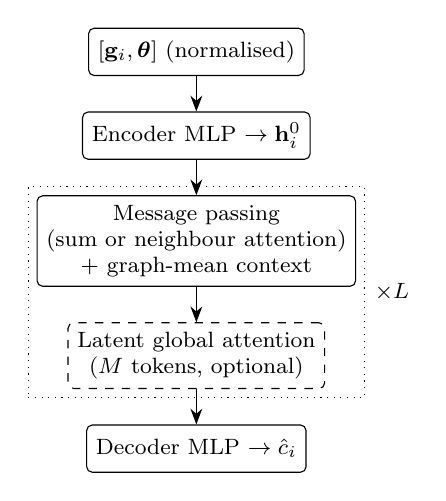
\begin{tikzpicture}[
  node distance=4.5mm,
  blk/.style={draw, rounded corners=2pt, minimum width=2.6cm, minimum height=6mm, align=center, font=\footnotesize},
  opt/.style={blk, dashed},
  >={Stealth[length=2mm]}]
\node[blk] (in) {$[\mathbf{g}_i,\boldsymbol{\theta}]$ (normalised)};
\node[blk, below=of in] (enc) {Encoder MLP $\to\mathbf{h}_i^{0}$};
\node[blk, below=of enc] (mp) {Message passing\\(sum or neighbour attention)\\+ graph-mean context};
\node[opt, below=of mp] (lat) {Latent global attention\\($M$ tokens, optional)};
\node[blk, below=of lat] (dec) {Decoder MLP $\to\hat{c}_i$};
\node[draw, dotted, inner sep=3pt, fit=(mp)(lat), label={[font=\footnotesize]east:$\times L$}] {};
\draw[->] (in) -- (enc);
\draw[->] (enc) -- (mp);
\draw[->] (mp) -- (lat);
\draw[->] (lat) -- (dec);
\end{tikzpicture}
\caption{Encode--process--decode architecture. Each of the $L=3$ processing
stages contains one residual message-passing block and, optionally, one latent
attention block. All attention is computed separately per design.}
\label{fig:arch}
\end{figure}

\subsection{Base Message-Passing GNN}
The model (Fig.~\ref{fig:arch}) encodes
$\mathbf{h}^0_i=\mathrm{MLP}_\mathrm{enc}([\mathbf{g}_i,\boldsymbol{\theta}])$
with a two-layer MLP, applies $L$ residual blocks, and decodes with a two-layer
MLP. In block $\ell$, for each directed edge $j\!\to\!i$,
\begin{align}
\mathbf{m}_{j\to i}&=\phi_e\big([\mathbf{h}_j,\mathbf{h}_i,\mathbf{e}_{ji}]\big),\\
\mathbf{a}_i&=\textstyle\sum_{j\in\mathcal{N}(i)}\mathbf{m}_{j\to i},\\
\mathbf{h}_i&\leftarrow\mathbf{h}_i+\phi_n\big([\mathbf{h}_i,\mathbf{a}_i,\bar{\mathbf{h}}_{g(i)}]\big),
\end{align}
where $\phi_e,\phi_n$ are Linear--LayerNorm--ReLU--Linear MLPs and
$\bar{\mathbf{h}}_{g}$ is the mean node state of the design (graph) $g$
containing node $i$. The graph mean provides a uniform global context but
cannot transmit \emph{localised} information across the domain. With
$L=3$, purely local information reaches only three hops, far smaller than the
graph diameter of meshes with $4\times10^3$--$1.5\times10^4$ cells.

\subsection{Edge-Aware Neighbour Attention}
Optionally, sum aggregation is replaced by $H$-head attention. Scores are
$\mathbf{s}_{j\to i}=\psi([\mathbf{h}_j,\mathbf{h}_i,\mathbf{e}_{ji}])\in\mathbb{R}^H$
with $\psi$ a Linear--LeakyReLU(0.2)--Linear MLP. A numerically stable segment
softmax over the incoming edges of each node gives
$\alpha^k_{j\to i}$, and the edge message $\mathbf{m}_{j\to i}$ is split into
$H$ chunks of width $d/H$ that act as values:
\begin{equation}
\mathbf{a}^k_i=\textstyle\sum_{j\in\mathcal{N}(i)}\alpha^k_{j\to i}\,\mathbf{m}^k_{j\to i}.
\end{equation}
Using the learned message as the value was a correction: an earlier draft had
separate value projections that received no gradient, which a gradient test
detected. Note that a convex combination discards the node-degree information
that sum aggregation retains. Cost is $\mathcal{O}(|E|d)$, the same order as
plain message passing, and this does not enlarge the receptive field.

\subsection{Latent-Token Global Attention}
\label{sec:latent}
To exchange localised information globally, an optional block follows each
message-passing layer. It holds $M$ learned tokens
$\mathbf{T}^0\in\mathbb{R}^{M\times d}$ shared across designs. For one design
with cell states $\mathbf{H}\in\mathbb{R}^{N\times d}$,
$\tilde{\mathbf{H}}=\mathrm{LN}_c(\mathbf{H})$,
\begin{align}
\mathbf{T}&=\mathbf{T}^0+\mathrm{MHA}_r\big(\mathrm{LN}_t(\mathbf{T}^0),\tilde{\mathbf{H}},\tilde{\mathbf{H}}\big)
&&\text{(cells$\to$tokens)}\\
\mathbf{T}&\leftarrow\mathbf{T}+\mathrm{MHA}_s\big(\mathrm{LN}_t(\mathbf{T}),\cdot,\cdot\big)
&&\text{(token self-attn.)}\\
\mathbf{T}&\leftarrow\mathbf{T}+\mathrm{FFN}_t(\mathbf{T}),\\
\mathbf{H}&\leftarrow\mathbf{H}+\mathrm{MHA}_w\big(\tilde{\mathbf{H}},\mathrm{LN}_t(\mathbf{T}),\mathrm{LN}_t(\mathbf{T})\big)
&&\text{(tokens$\to$cells)}\\
\mathbf{H}&\leftarrow\mathbf{H}+\mathrm{FFN}_c(\mathbf{H}),
\end{align}
where the FFNs are pre-LayerNorm, width-$2d$, GELU MLPs and the MHA layers are
PyTorch \texttt{nn.MultiheadAttention} with $H=4$ heads and
\texttt{need\_weights=False}. Every cell can influence every other cell within
one block through the tokens.

\textbf{Graph isolation.} Mini-batches concatenate designs, so the block loops
over design identifiers and attends within each design separately, including
when batch membership is non-contiguous. Without this, information would leak
between designs.

\textbf{Complexity and the deliberate compromise.} Full cell-to-cell attention
requires $N^2$ scores per head; at $N=5\times10^4$ this is $2.5\times10^9$
pairs. The latent block needs $2NM+M^2$ scores, i.e.\
$\approx3.2\times10^6+1{,}024$ pairs for $M=32$. The bottleneck can discard
spatial detail; it is \emph{not} equivalent to unrestricted all-cell attention
and is not a reproduction of PhysicsAI. The token count $M$ is also not the
same setting as PhysicsAI's 300 sample points.
Full attention was deferred, not rejected on accuracy grounds.

\subsection{Activation Variants}
A model-level option replaces every hidden nonlinearity by $\tanh$: ReLU in the
encoder, decoder, $\phi_e$ and $\phi_n$; GELU in the token and cell FFNs; and
LeakyReLU in the neighbour-attention score MLP. Softmax inside attention is
unchanged. Because $\tanh$ has no parameters, the parameter count and the
sequence of random initialisation draws are unchanged; with identical seeds the
two activation variants start from identical weights and visit designs in the
same order. The activation is stored in checkpoints; older checkpoints default
to the original activations.

\subsection{Variants and Parameter Counts}
All volume models use width $d$, $L=3$ blocks, 5 node features, 4 edge
features, 3 parameters and one output (Table~\ref{tab:archs}). Parameter-matched
widths were found by search: the plain GNN over widths 40--80 and the neighbour
model over head-divisible widths 40--128, minimising the absolute difference to
the latent-attention model's 92{,}097 parameters. The nearest legal neighbour
width (56) is 3.32\,\% above the target.

\begin{table}[!t]
\centering
\caption{Volume Architectures (All $L=3$, $H=4$)}
\label{tab:archs}
\setlength{\tabcolsep}{3.5pt}
\begin{tabular}{lrrrr}
\toprule
Name & $d$ & Tokens & Aggregation & Params \\
\midrule
\texttt{gnn32} & 32 & -- & sum & 25{,}089 \\
\texttt{gnn\_parameter\_matched} & 62 & -- & sum & 91{,}389 \\
\texttt{latent\_attention32} & 32 & 32 & sum & 92{,}097 \\
\texttt{neighbor\_attention32} & 32 & -- & attention & 32{,}109 \\
\texttt{neighbor\_attn\_param\_matched} & 56 & -- & attention & 95{,}157 \\
\bottomrule
\end{tabular}\\[2pt]
\footnotesize Each also exists as a \texttt{\_tanh} variant with identical parameter count.
\end{table}

The counts decompose exactly: each latent block adds
$1{,}024$ (tokens) $+128$ (two LayerNorms) $+3\times4{,}224$ (MHA) $+2\times4{,}256$
(FFNs) $=22{,}336$ parameters, and each neighbour-attention score MLP adds
$2{,}340$. Parameter matching controls only parameter count, not FLOPs,
memory or runtime.

% =============================================================================
\section{Training Objectives}
\label{sec:losses}
% =============================================================================
\subsection{Surface Model: Field and Integrated Drag}
The surface model predicts the pressure and streamwise wall-shear coefficients
on each wall face. Drag is a differentiable reduction
\begin{equation}
F_D=\textstyle\sum_f\big(p_f\,n_{x,f}+\tau_{x,f}\big)A_f,
\end{equation}
and training minimises
\begin{equation}
\mathcal{L}=\mathrm{MSE}(\hat{\mathbf{c}},\mathbf{c})+\lambda(t)\,
\mathbb{E}_g\Big[\big((\hat F_{D,g}-F_{D,g})/F_{D,g}\big)^2\Big],
\end{equation}
with $\lambda$ ramped linearly from 0 to 0.5 over the first 20\,\% of epochs.
The relative drag error weights a 4\,N slender body and a 120\,N bluff body
equally. An optional per-face weighting by drag sensitivity ($|n_x|A$ for
pressure, $A$ for shear) is implemented but disabled (mix 0). Settings: width
64, four layers, global context, batch 4, 600 epochs, AdamW, five folds.

\subsection{Volume Model: Area-Weighted Loss}
For residuals $r_i=\hat c_i-c_i$ in normalised units,
\begin{equation}
\mathcal{L}_\mathrm{area}=\frac{\sum_i A_i r_i^2}{\sum_i A_i},
\end{equation}
which approximates the domain integral of squared error and prevents the dense
near-wall mesh from dominating. Table~\ref{tab:data} shows the consequence:
the near-wall region receives under 2\,\% of the weight.

\subsection{Volume Model: Near-Body-Balanced Loss}
Let $\delta=0.05$\,m and $\mathcal{B}_g=\{i\in g: d_i\le\delta\}$. Per design $g$,
\begin{equation}
w_i=(1-\mu)\frac{A_i}{\sum_{k\in g}A_k}
+\mu\frac{A_i\,\mathbb{1}[i\in\mathcal{B}_g]}{\sum_{k\in\mathcal{B}_g}A_k},
\quad
\mathcal{L}_\mathrm{nb}=\frac1G\sum_{g}\sum_{i\in g}w_i r_i^2,
\end{equation}
with $\mu=0.5$, i.e.\ half the weight on the whole-domain area-average and half
on the near-body area-average. If a design had no near-body cells, its domain
weights would be used. Membership depends only on geometry (wall distance),
never on the target pressure, so the weighting does not leak target
information. Per-design normalisation also gives each design equal weight
regardless of its cell count.

\subsection{Optimisation}
AdamW~\cite{loshchilov2019} (learning rate $10^{-3}$, weight decay $10^{-5}$),
cosine annealing~\cite{loshchilov2017sgdr} to $10^{-5}$, one design per batch,
CPU execution, single thread. In the 40-epoch studies the cosine period equals
the run length. In the nested studies the period is the 1{,}000-epoch maximum;
the consequences are discussed in Section~\ref{sec:discussion}.

% =============================================================================
\section{Evaluation Protocols and Metrics}
\label{sec:protocols}
% =============================================================================
\subsection{Five-Fold Cross-Validation}
Designs are permuted with seed 0 and assigned to five folds of six by striding.
Fold $k$ uses training seed $k-1$. Scalers are refitted per fold. The epoch
count is identical for cross-validation and the final fit (an earlier mismatch
was removed). Fold~2 holds out Designs~1, 3, 4, 13, 14 and 26.

\subsection{Fixed-Fold Diagnostics}
Loss and first attention experiments reuse fold~2: 24 training and six held-out
designs, seed 1, 40 epochs. Cached reference predictions were reused rather than
retrained, and validated against the current CFD export before plotting.

\subsection{Nested Selection Protocol}
\label{sec:nested}
To separate checkpoint selection from evaluation:
\begin{enumerate}
\item Outer split: fold~2 (24 outer-training, six outer-test designs).
\item Inner split: a seeded (2026) 80/20 permutation of the 24 gives 19
inner-training and five inner-validation designs
(Designs~9, 11, 15, 21, 27).
\item Scalers are fitted on the 19 inner-training designs only.
\item Train for at most 1{,}000 epochs; every 10 epochs compute the
near-body-balanced normalised loss on the inner-validation designs and save the
model (with its scalers) when it improves.
\item Stop once at least 100 epochs have elapsed and eight consecutive
checks brought no improvement.
\item Reload the best checkpoint and evaluate it once on the six outer designs.
\end{enumerate}
The outer designs are never used for gradient updates or checkpoint selection.
However, they had been inspected in earlier experiments and are reused across
all architecture comparisons, so results are \emph{exploratory}, not an unbiased
test. Every report records \texttt{outer\_test\_previously\_inspected=true}.

\subsection{Metrics}
All metrics are computed in pascals, weighted by cell area. For design $g$,
\begin{equation}
\RMSE_g=\sqrt{\frac{\sum_{i\in g}A_i(\hat p_i-p_i)^2}{\sum_{i\in g}A_i}},
\end{equation}
and the near-body RMSE restricts the sums to $\mathcal{B}_g$. We report the
mean, median and worst per-design RMSE, the mean near-body RMSE, per-design
$R^2_g$ (area-weighted), and a pooled $R^2$ whose total variance is assembled
exactly from per-design statistics via the law of total variance,
$\mathrm{SS}_\mathrm{tot}=\sum_g\big[V_g+A_g(\mu_g-\mu)^2\big]$.
Pooled $R^2$ is dominated by between-design variance (large, fast bodies have
large pressures) and can be high even when individual fields are poor; the
per-design means are therefore preferred. The median uses the conventional
definition (an earlier use of PyTorch's lower-middle median was corrected).

\subsection{Explicit Multi-Criterion Ranking}
To make trade-offs explicit, each model $m$ receives a weighted relative regret
\begin{equation}
R(m)=\sum_k \frac{w_k}{\sum_{k'}w_{k'}}\Big(\frac{x_{m,k}}{\min_{m'}x_{m',k}}-1\Big)
\end{equation}
over $k\in\{$mean RMSE, mean near-body RMSE, worst RMSE$\}$ with profiles
\emph{balanced} (0.4/0.4/0.2), \emph{whole-domain} (0.6/0.2/0.2) and
\emph{near-body only} (0/1/0). Weights express priorities, not a calibrated
utility or statistical confidence.

\subsection{Visual Protocol}
Every experiment produces per-design three-panel images (CFD, reference model,
new model) on a \emph{shared} pressure colour scale, drawn on the true cell
polygons and annotated with whole-domain and near-body errors. This protocol was
adopted after aggregate metrics were found to overstate the visual quality of
early models (Section~\ref{sec:exp_cv}).

% =============================================================================
\section{Experiments and Results}
\label{sec:results}
% =============================================================================
The experiments are presented chronologically; each subsection states the
hypothesis, protocol, measurement and decision.

\subsection{Surface Drag Model (Preliminary Stage)}
The project began with the surface model of Section~\ref{sec:losses}. Its
development history added a direct drag loss and $k$-fold validation and
removed density as an output (density is constant). Checkpoints were trained on
all designs; the validation script therefore labels its plots as
\emph{reconstructions} and offers a separate hold-out mode that retrains without
the selected design. Quantitative cross-validated surface results were not
recorded in the research log and are not reported here. The surface stage is
retained in the code but was not developed further; the remainder of this
report concerns the volume pressure field.

\subsection{Target Scaling and Geometric Features (Five-Fold CV)}
\label{sec:exp_cv}
\hyp{coefficient targets remove speed-dependent scaling; wall distance and
dimensionless edge geometry give useful context without adding layers.}
Protocol: width 32, three layers, 40 epochs, area loss, matched fold membership
and seeds. Results are in Table~\ref{tab:cv}.

\begin{table}[!t]
\centering
\caption{Five-Fold Cross-Validation, 30 Designs, 40 Epochs}
\label{tab:cv}
\setlength{\tabcolsep}{3pt}
\begin{tabular}{lrrrrr}
\toprule
Variant & Mean & Worst & Mean nb & Pooled & Mean \\
 & RMSE & RMSE & RMSE & $R^2$ & $R^2_g$ \\
\midrule
Raw pressure & 6.621 & 19.204 & 27.147 & 0.9634 & 0.8048 \\
Coefficient & 5.710 & 16.834 & \textbf{24.903} & 0.9742 & \textbf{0.8359} \\
Coef.\ + geometry & \textbf{5.626} & 16.894 & 25.276 & \textbf{0.9745} & 0.8263 \\
\bottomrule
\end{tabular}\\[2pt]
\footnotesize RMSE in Pa; nb = near-body ($d\le0.05$\,m).
\end{table}

Coefficient targets reduced mean RMSE by 13.8\,\%, near-body RMSE by 8.3\,\%
and worst-design RMSE by 12.3\,\%. Adding geometric features gave a further
1.5\,\% in mean RMSE but a 1.5\,\% increase in near-body RMSE and a lower mean
$R^2_g$; the evidence for the features is therefore weak, and they were kept
mainly because wall distance is required by the near-body loss.
The minimum per-design $R^2_g$ (0.17 raw, 0.39 coefficient, 0.36 geometry)
reveals that pooled $R^2\approx0.97$ hides poorly predicted designs.

\textbf{Problem recorded.} Inspection of held-out fields
(Fig.~\ref{fig:cvfield}) was much less convincing than the pooled metrics, and
the gains were initially described too positively. Visual evidence became a
mandatory part of every subsequent comparison.

\begin{figure}[!t]
\centering
\includegraphics[width=\columnwidth]{validation_results/volume/validation_volume_Design_1_geometry.png}
\caption{Held-out (fold~2) prediction for Design\_1 with the coefficient +
geometry model under five-fold CV. The broad field is reproduced but near-body
structure is not.}
\label{fig:cvfield}
\end{figure}

\subsection{Capacity Diagnosis: Single-Design Reconstruction}
\label{sec:exp_overfit}
\hyp{the width-32, three-layer GNN cannot represent the field at all.}
We trained on Design\_1 alone for 1{,}200 optimiser steps with the area loss.
Reconstruction RMSE was 0.242\,Pa, near-body RMSE 1.94\,Pa, $R^2=0.9986$
(Fig.~\ref{fig:overfit}). The network can therefore \emph{represent} one field;
this is reconstruction, not validation, and does not establish that the same
capacity suffices for all designs jointly or for generalisation.

\begin{figure}[!t]
\centering
\includegraphics[width=\columnwidth]{volume_results/diagnosis/overfit_area/Design_1.png}
\caption{Single-design reconstruction of Design\_1 (training data; \emph{not}
validation).}
\label{fig:overfit}
\end{figure}

\subsection{Near-Body-Balanced Loss (Fold 2)}
\label{sec:exp_loss}
\hyp{the area loss neglects the near-wall region because it holds 1.73\,\% of
the area.} Same architecture, seed, 24 training designs and 40 epochs; only the
loss changed; the cached area-loss predictions were reused.

\begin{table}[!t]
\centering
\caption{Loss Comparison on Fold 2 (Six Held-Out Designs)}
\label{tab:loss}
\begin{tabular}{lrr}
\toprule
Metric & Area loss & Near-body loss \\
\midrule
Mean RMSE [Pa] & \textbf{4.997} & 5.402 \\
Worst RMSE [Pa] & \textbf{5.918} & 7.767 \\
Mean near-body RMSE [Pa] & 29.597 & \textbf{14.704} \\
Pooled $R^2$ & \textbf{0.8903} & 0.8682 \\
Mean $R^2_g$ & \textbf{0.7001} & 0.6965 \\
Min $R^2_g$ & 0.3630 & \textbf{0.4222} \\
\bottomrule
\end{tabular}
\end{table}

Near-body RMSE fell by 50.3\,\% while whole-domain RMSE rose by 8.1\,\%
(Table~\ref{tab:loss}, Fig.~\ref{fig:loss}). This is a trade-off on one fold,
not a full-CV improvement. Defaults were not changed; the near-body loss was
adopted for all later experiments because near-body accuracy governs loads.

\begin{figure*}[!t]
\centering
\includegraphics[width=0.95\textwidth]{volume_results/diagnosis/fold_near_body/Design_1_loss_comparison.png}
\caption{Design\_1, fold~2: CFD (left), area loss (centre), near-body-balanced
loss (right), on a common pressure scale.}
\label{fig:loss}
\end{figure*}

\subsection{First Latent-Attention Experiment (Fold 2, 40 Epochs)}
\label{sec:exp_att1}
\hyp{global token exchange improves pressure fields beyond three-hop locality.}
Protocol identical to Section~\ref{sec:exp_loss} with the near-body loss; only
the 32-token, four-head blocks were added. Before the run, 28 regression tests
verified graph isolation (perturbing one design leaves another unchanged),
node-permutation equivariance, gradient flow from one cell to a distant cell,
gradients through every attention parameter, disabled-mode compatibility with
old checkpoints, and checkpoint round trips.

\begin{table}[!t]
\centering
\caption{First Attention Experiment, Fold 2, 40 Epochs}
\label{tab:att1}
\setlength{\tabcolsep}{4pt}
\begin{tabular}{lrrrr}
\toprule
 & \multicolumn{2}{c}{No attention} & \multicolumn{2}{c}{Latent attention} \\
Design & RMSE & nb RMSE & RMSE & nb RMSE \\
\midrule
Design\_1 & 4.904 & 19.339 & \textbf{4.677} & \textbf{16.130} \\
Design\_3 & 7.767 & 15.139 & \textbf{7.083} & \textbf{13.733} \\
Design\_4 & \textbf{3.841} & 6.319 & 5.153 & \textbf{5.430} \\
Design\_13 & \textbf{4.751} & 11.389 & 5.056 & \textbf{10.877} \\
Design\_14 & \textbf{5.066} & \textbf{21.911} & 6.311 & 22.310 \\
Design\_26 & \textbf{6.085} & \textbf{14.130} & 8.292 & 14.842 \\
\midrule
Mean & \textbf{5.402} & 14.704 & 6.095 & \textbf{13.887} \\
\bottomrule
\end{tabular}
\end{table}

\textbf{Result: mixed.} Mean near-body RMSE improved 5.6\,\% but mean
whole-domain RMSE worsened 12.8\,\%, improving on only two of six designs
(Table~\ref{tab:att1}). Visually, Design\_1 showed better localisation but a
broader pressure pattern than CFD; Design\_26 worsened
(Fig.~\ref{fig:att1}). The model was reloaded and reproduced all six saved
predictions within $10^{-5}$. Attention remained optional and off by default.
This run changed parameter count (25{,}089$\rightarrow$92{,}097) and used a short
fixed schedule, so it could not isolate the cause; this motivated the nested
study.

\begin{figure*}[!t]
\centering
\includegraphics[width=0.95\textwidth]{volume_results/diagnosis/fold_attention/Design_26_attention_comparison.png}
\caption{A worsened case from the first attention run (Design\_26): CFD,
near-body GNN without attention, GNN with latent attention.}
\label{fig:att1}
\end{figure*}

\subsection{Nested Architecture Study}
\label{sec:exp_nested}
\hyp{with a longer budget and validation-based checkpoint selection, global
communication helps beyond what extra capacity provides.}
Four architectures were trained under the protocol of Section~\ref{sec:nested}
with identical split, seed, loss, optimiser and stopping rule
(Table~\ref{tab:nested}, per-design results in Table~\ref{tab:perdesign}).

\begin{table*}[!t]
\centering
\caption{Nested Study on Outer Fold 2: Inner-Validation-Selected Checkpoints Evaluated on Six Outer Designs}
\label{tab:nested}
\begin{tabular}{lrrrrrrrrr}
\toprule
Architecture & Params & Best & Stop & Inner-val & Mean & Worst & Mean nb & Pooled & Mean \\
 & & epoch & epoch & loss & RMSE & RMSE & RMSE & $R^2$ & $R^2_g$ \\
\midrule
\texttt{gnn32} & 25{,}089 & 50 & 130 & 0.02944 & 4.966 & 6.722 & 19.928 & 0.8903 & 0.6777 \\
\texttt{gnn\_parameter\_matched} & 91{,}389 & 170 & 250 & 0.02616 & 3.248 & 5.515 & 14.048 & 0.9452 & 0.7835 \\
\texttt{latent\_attention32} & 92{,}097 & 160 & 240 & \textbf{0.01303} & 2.984 & 4.059 & 11.963 & 0.9584 & 0.8663 \\
\texttt{neighbor\_attention32} & 32{,}109 & 180 & 260 & 0.01600 & 3.427 & 5.168 & 11.952 & 0.9451 & 0.8146 \\
\texttt{neighbor\_attn\_param\_matched} & 95{,}157 & 120 & 200 & 0.02020 & 3.472 & 5.639 & 12.873 & 0.9391 & 0.7681 \\
\midrule
\texttt{latent\_attention32\_tanh} & 92{,}097 & 260 & 340 & 0.01399 & \textbf{2.924} & \textbf{3.967} & \textbf{9.348} & \textbf{0.9600} & \textbf{0.8687} \\
\texttt{neighbor\_attention32\_tanh} & 32{,}109 & 80 & 160 & 0.01636 & 3.395 & 4.347 & 12.765 & 0.9484 & 0.8574 \\
\texttt{neighbor\_attn\_param\_matched\_tanh} & 95{,}157 & \multicolumn{8}{c}{\emph{run in progress at the time of writing; no outer results}} \\
\bottomrule
\end{tabular}\\[2pt]
\footnotesize RMSE in Pa. One seed (2026), one outer fold whose designs were previously inspected. Stop epoch = last trained epoch.
\end{table*}

\begin{table*}[!t]
\centering
\caption{Per-Design Outer-Fold Errors, Whole-Domain RMSE / Near-Body RMSE [Pa]}
\label{tab:perdesign}
\setlength{\tabcolsep}{4pt}
\begin{tabular}{lcccccc}
\toprule
Architecture & Design\_1 & Design\_3 & Design\_4 & Design\_13 & Design\_14 & Design\_26 \\
\midrule
\texttt{gnn32} & 4.93 / 25.85 & 5.10 / 15.50 & 4.97 / 14.90 & 3.80 / 13.28 & 6.72 / 36.36 & 4.28 / 13.67 \\
\texttt{gnn\_parameter\_matched} & 5.52 / 24.94 & \textbf{2.79} / 8.85 & 2.30 / 6.66 & \textbf{1.52} / 5.16 & 4.95 / 32.90 & 2.42 / 5.77 \\
\texttt{latent\_attention32} & 3.81 / 21.34 & 3.21 / 7.55 & 3.06 / 8.16 & 1.61 / 5.94 & 4.06 / 24.52 & \textbf{2.16} / 4.27 \\
\texttt{neighbor\_attention32} & 4.06 / 19.16 & 3.00 / 9.41 & 1.92 / 6.55 & 2.97 / 8.50 & 5.17 / 24.59 & 3.45 / 3.50 \\
\texttt{neighbor\_attn\_param\_matched} & 5.64 / 27.93 & 2.93 / 8.97 & 2.17 / 3.40 & 1.84 / 5.95 & 5.14 / 26.72 & 3.11 / 4.27 \\
\texttt{latent\_attention32\_tanh} & 3.97 / \textbf{17.99} & 3.50 / \textbf{6.37} & \textbf{1.60} / \textbf{2.37} & 2.22 / \textbf{5.09} & \textbf{3.67} / \textbf{21.16} & 2.59 / \textbf{3.11} \\
\texttt{neighbor\_attention32\_tanh} & \textbf{3.42} / 18.93 & 4.35 / 9.47 & 2.54 / 4.52 & 2.71 / 6.00 & 4.15 / 32.90 & 3.20 / 4.77 \\
\bottomrule
\end{tabular}\\[2pt]
\footnotesize Bold: column minimum. Design\_1 and Design\_14 have $\pdone\approx0.05$.
\end{table*}

\textbf{Capacity.} The parameter-matched GNN improved on \texttt{gnn32} by
34.6\,\% in mean RMSE and 29.5\,\% in near-body RMSE. Capacity is a major factor;
the first attention experiment conflated it with architecture.

\textbf{Global attention versus its capacity control.} At near-identical
parameter count, \texttt{latent\_attention32} improved on
\texttt{gnn\_parameter\_matched} by 8.1\,\% in mean RMSE, 14.8\,\% in near-body
RMSE and 26.4\,\% in worst-design RMSE, and achieved the lowest inner-validation
loss by a wide margin (0.0130 versus 0.0262). It is, however, not FLOP-matched.

\textbf{Neighbour attention.} At only 32{,}109 parameters,
\texttt{neighbor\_attention32} matched the latent model's near-body RMSE
(11.952 versus 11.963\,Pa, a negligible 0.01\,Pa) but was 0.44\,Pa worse in mean
RMSE and 1.11\,Pa worse in worst-design RMSE.

\textbf{Parameter-matched neighbour attention.} Widening to 56 did not help:
mean, near-body and worst-design RMSE were 1.3\,\%, 7.7\,\% and 9.1\,\% worse than
width 32, and its inner-validation loss was higher. We do not conclude that
parameter count caused the difference; one seed cannot separate it from
optimisation variance.

All selected checkpoints were reloaded and matched their recorded epochs and
scalers. Validation curves (e.g.\ Fig.~\ref{fig:valcurve}) and three-panel
images exist for every model and design.

\subsection{Activation Study: $\tanh$}
\label{sec:exp_tanh}
\hyp{smooth, bounded $\tanh$ activations suit smooth pressure fields better than
piecewise-linear ReLU; this is a hypothesis, not a known property.}
Each $\tanh$ model was compared only with its own activation baseline, matched in
split, seed, architecture dimensions, initial weights and data order.

\textbf{Latent attention.} The first run stopped for an unknown reason
before writing results (best checkpoint at epoch 70, loss 0.02330; no optimiser
state, so no exact resume). That partial artifact was preserved and the run was
restarted from epoch 1 in a separate directory. The restarted run stopped at
epoch 340 and selected epoch 260. Mean near-body RMSE improved by 21.9\,\%
(11.96$\rightarrow$9.35\,Pa) with improvements on all six designs; mean
whole-domain RMSE improved by 2.0\,\% despite worsening on four of six designs,
driven mainly by Design\_4 (3.06$\rightarrow$1.60\,Pa,
Fig.~\ref{fig:tanh4}). Notably the $\tanh$ model's \emph{inner-validation} loss
was \emph{higher} (0.01399 versus 0.01303), so the outer improvement is not
predicted by the selection criterion. Design\_14 (Fig.~\ref{fig:tanh14})
improves numerically but shows streak artefacts upstream of the body.

\textbf{Width-32 neighbour attention.} Stopped at epoch 160, selected epoch 80
(baseline 180). Mean RMSE improved 0.9\,\% and worst-design RMSE 15.9\,\%, but
near-body RMSE worsened 6.8\,\%, dominated by Design\_14
(24.59$\rightarrow$32.90\,Pa).

\textbf{Parameter-matched neighbour attention.} At the time of writing this run
is active (dataset loaded; best checkpoint last updated during training); no
outer-fold results exist and none are reported.

\begin{figure*}[!t]
\centering
\includegraphics[width=0.95\textwidth]{volume_results/architecture_tanh_restart/latent_attention32_tanh/Design_4_comparison.png}
\caption{Design\_4: CFD, latent attention (ReLU/GELU), latent attention ($\tanh$).
Errors 3.06/8.16\,Pa and 1.60/2.37\,Pa (whole/near-body).}
\label{fig:tanh4}
\end{figure*}

\begin{figure*}[!t]
\centering
\includegraphics[width=0.95\textwidth]{volume_results/architecture_tanh_restart/latent_attention32_tanh/Design_14_comparison.png}
\caption{Design\_14 ($\pdone=0.0505$), the hardest outer design: CFD, latent
attention, latent attention with $\tanh$. Both models under-resolve the small
body's stagnation and suction peaks; $\tanh$ introduces upstream streaks.}
\label{fig:tanh14}
\end{figure*}

\begin{figure}[!t]
\centering
\includegraphics[width=\columnwidth]{volume_results/architecture_tanh_restart/latent_attention32_tanh/validation_curve.png}
\caption{Training and inner-validation loss for \texttt{latent\_attention32\_tanh}.
The validation loss fluctuates by a factor of about three between checks.}
\label{fig:valcurve}
\end{figure}

\subsection{Ranking}
\label{sec:exp_rank}
Table~\ref{tab:rank} applies the regret ranking to the seven completed models.
The ranking files saved by the project cover the first five; the seven-model
ranking was computed for this report with the same function, without
retraining. \texttt{latent\_attention32\_tanh} has zero regret in every profile
because it is best on all three criteria. Among the original five, latent
attention won the balanced and whole-domain profiles and width-32 neighbour
attention won near-body-only by 0.011\,Pa, effectively a tie.

\begin{table}[!t]
\centering
\caption{Weighted Relative Regret (Lower Is Better), Seven Models}
\label{tab:rank}
\setlength{\tabcolsep}{3.5pt}
\begin{tabular}{lrrr}
\toprule
Model & Balanced & Whole & Near-body \\
\midrule
\texttt{latent\_attention32\_tanh} & \textbf{0.000} & \textbf{0.000} & \textbf{0.000} \\
\texttt{latent\_attention32} & 0.125 & 0.073 & 0.280 \\
\texttt{neighbor\_attention32\_tanh} & 0.230 & 0.189 & 0.366 \\
\texttt{neighbor\_attention32} & 0.241 & 0.220 & 0.279 \\
\texttt{neighbor\_attn\_param\_matched} & 0.310 & 0.272 & 0.377 \\
\texttt{gnn\_parameter\_matched} & 0.324 & 0.245 & 0.503 \\
\texttt{gnn32} & 0.871 & 0.784 & 1.132 \\
\bottomrule
\end{tabular}
\end{table}

% TODO(rough draft): polish this subsection; added 2026-11-22.
\subsection{Scale Invariance, Stratified Selection and Transolver}
\label{sec:exp_transolver}
\textbf{Body-scaled inputs failed.} Scaling positions and wall distance by the
body's streamwise length $L_\mathrm{ref}$ (and dropping cell size from node
inputs) worsened the latent model to 5.35\,Pa mean and 10.01\,Pa worst-design
RMSE. Diagnosis: body length varies $12.7\times$ across designs but the
$3\times1$\,m channel is fixed, so small bodies reach $x/L_\mathrm{ref}\approx48$
while training never exceeded 16.7; 70--88\,\% of their fluid area lay outside
the training input range. The flow is confined, so blockage and distance to the
outlet are missing dimensionless groups when only $L_\mathrm{ref}$ is used.

\textbf{Two fixes.} (i) A \emph{two-scale} input: positions normalised by the
fluid-domain box (bounded in $[0,1]$), wall distance by $L_\mathrm{ref}$, and
blockage plus a Reynolds proxy as design inputs. (ii) A stratified inner split
that draws one validation design per body-length stratum, so small bodies appear
in training. The outer six test designs are unchanged.

\textbf{Transolver.} We implemented Transolver~\cite{wu2024transolver}
(physics-attention over learned soft slices; mesh edges unused) as an external
benchmark and trained it under the identical nested protocol.
Table~\ref{tab:h2h} is the running head-to-head table; every subsequent
addition is appended as a new row on the same split.

\begin{table}[!t]
\centering
\caption{Running Head-to-Head Comparison (Stratified Fold~2, Six Outer Designs)}
\label{tab:h2h}
\setlength{\tabcolsep}{3pt}
\begin{tabular}{lrrrrr}
\toprule
Model & RMSE & Near-wall & $C_D$ err. & Mem. & Inf. \\
 & [Pa] & [Pa] & [\%] & [GB] & time \\
\midrule
Transolver (CPU benchmark) & 1.39 & 2.77 & n/m & n/m & n/m \\
Transolver (GPU rerun) & \textbf{1.11} & \textbf{2.02} & n/m & n/m & n/m \\
Two-scale latent GNN & 2.37 & 8.22 & n/m & n/m & n/m \\
Latent GNN (geometry) & 3.32 & 10.87 & n/m & n/m & n/m \\
Latent GNN (geometry, GPU) & 2.41 & 6.84 & n/m & n/m & n/m \\
\bottomrule
\end{tabular}
\\[2pt]
\footnotesize Near-wall: wall distance $\le0.05$\,m. n/m: not yet measured.
\end{table}

Two-scale inputs improved the matched latent GNN on all six designs in
whole-domain RMSE (mean $-28$\,\%, worst $-38$\,\%), but Transolver, with
27{,}757 parameters versus 92{,}161, is better on every metric and roughly
$3\times$ better near the wall. The hypothesis that face-to-face message passing
would win near walls is not supported. Caveats: the two-scale run used a
body-relative near-wall loss band ($0.15\,L_\mathrm{ref}$) while the others used
0.05\,m; Transolver used geometry inputs; one seed on a reused fold.
Fig.~(TODO) should show Design\_14 with CFD, both GNNs and Transolver on a
shared scale (\texttt{volume\_results/stratified\_20261122/transolver32/}).

The same Transolver protocol was rerun on an NVIDIA RTX PRO 4000 laptop GPU.
It reached its best validation checkpoint at epoch 600 and stopped at epoch 680,
compared with epochs 250 and 330 in the earlier CPU run. Mean held-out RMSE
was 1.11\,Pa and near-wall RMSE was 2.02\,Pa. These single runs use different
devices and PyTorch builds, so the accuracy difference is not evidence that the
GPU itself improves accuracy. A common-scale comparison of actual CFD, the CPU
reference and the GPU rerun is saved as
\texttt{volume\_results/gpu\_transolver\_full\_20261122/Design\_1\_benchmark\_comparison.png}.

A geometry-input latent GNN rerun on the same GPU stopped at epoch 650, with
its best checkpoint at epoch 570. Its mean held-out and near-wall RMSE were
2.41\,Pa and 6.84\,Pa, respectively: lower than the earlier CPU latent run but
higher than the GPU Transolver run. Different checkpoints and PyTorch builds
confound this single-run comparison. A common-scale comparison with actual CFD,
the CPU latent model and GPU Transolver is saved as
\texttt{volume\_results/gpu\_latent\_attention\_geometry\_20261122/latent\_attention32/Design\_1\_benchmark\_comparison.png}.

\textbf{Decision.} Pure message-passing GNNs are retained only as references.
Further work improves Transolver one change at a time: two-scale inputs,
area-weighted slicing (discretisation-invariant slice averages), a corrected
learning-rate schedule, seeds and capacity, then conservation losses.

% =============================================================================
\section{Discussion}
\label{sec:discussion}
% =============================================================================
\subsection{What the Evidence Supports}
\begin{itemize}
\item \textbf{Physical scaling helps} (five-fold CV, all 30 designs held out
once): the most robust result in this report.
\item \textbf{Loss weighting determines where accuracy goes.} The near-body
loss trades a small whole-domain penalty for a large near-wall gain, which is
expected given the 1.73\,\% area fraction.
\item \textbf{Capacity matters}, and earlier comparisons that changed parameter
count were not interpretable as architecture effects.
\item \textbf{Global communication is promising}: the latent model beat its
parameter-matched control on every summary metric and on inner validation.
This is consistent with the elliptic nature of pressure, but rests on one seed
and one fold.
\end{itemize}

\subsection{Retrospective Finding: Parametric Extrapolation}
\label{sec:extrap}
While preparing this report we compared the parameter coverage of the nested
splits. The 19 inner-training designs span $\pdone\in[0.114,0.5]$; \emph{none}
has $\pdone<0.1$. All five designs with $\pdone\approx0.05$ fell outside
inner training: Designs~1 and 14 in the outer test and Designs~9, 15 and 21 in
inner validation. Consequently:
\begin{enumerate}
\item The two consistently worst outer designs (Design\_1 and Design\_14, with
near-body RMSE of 18--36\,Pa for every model) are extrapolations in shape space,
toward very small bodies whose high-gradient region spans few cells.
\item Three of five inner-validation designs are also extrapolations, so
checkpoint selection mostly rewards extrapolation behaviour rather than
interpolation accuracy.
\item In the 40-epoch fold-2 runs, Designs~9, 15 and 21 were in training; the
nested models had less coverage of this corner than the earlier references.
\end{enumerate}
This is a property of one random split, not a flaw in the code, but it
materially affects interpretation. The PhysicsAI external test domain
($\pdone\in[0.1,0.2]$) lies in the interior, so our hardest cases are harder
than that benchmark. A stratified or space-filling inner split would reduce
this effect.

\subsection{Confounds in the Architecture and Activation Comparisons}
\textbf{Learning-rate schedule.} The cosine period is the 1{,}000-epoch
maximum, but every nested run stopped by epoch 340. The learning rate at the
selected epochs was therefore still high: about $9.9\times10^{-4}$ at epoch 50,
$8.4\times10^{-4}$ at epoch 260, and never below $7.4\times10^{-4}$. Models
were effectively trained at a near-constant learning rate and selected from a
noisy trajectory; differences in stopping epoch translate into different
annealing states.

\textbf{Validation noise.} Five validation designs and a high learning rate
produce validation losses that fluctuate by about a factor of three between
consecutive checks (Fig.~\ref{fig:valcurve}). The selected epoch partly
reflects chance. The $\tanh$ latent model's better outer results despite a worse
inner-validation loss illustrate the weak coupling between the selection
signal and outer metrics on this split.

\textbf{Initialisation and data order.} Each architecture's mini-batch order
derives from the global seed after its own initialisation consumes random
numbers, so different architectures see different data orders. Only the
activation pairs are matched in both initialisation and order.

\textbf{Compute.} Parameter matching does not match FLOPs: the latent block
adds $\mathcal{O}(NMd)$ attention work, and the per-design Python loop adds
overhead. Wall-clock time was not recorded.

\textbf{Fold reuse.} The six outer designs were inspected in several prior
experiments and are reused for every comparison. Repeated comparison on a fixed
set induces selection bias~\cite{cawley2010}; reported differences of a few
percent are well within what this could produce.

\subsection{Visual Versus Aggregate Evidence}
Pooled $R^2$ above 0.95 coexists with per-design $R^2_g$ as low as 0.15.
Whole-domain RMSE is dominated by the large far-field area, where pressure is
smooth; near-body RMSE is several times larger and is where models differ
visibly. Shared-scale field images repeatedly revealed artefacts (broad
smearing, upstream streaks, under-resolved peaks) not evident from summaries.

% =============================================================================
\section{Limitations and Threats to Validity}
\label{sec:limits}
% =============================================================================
\begin{itemize}
\item One seed and one outer fold for every architecture/activation result;
no confidence intervals.
\item Outer designs previously inspected; results are exploratory.
\item Thirty designs total; 19 used for gradient updates in nested runs.
\item Inner split leaves the $\pdone\approx0.05$ corner uncovered
(Section~\ref{sec:extrap}).
\item No FLOP, memory or runtime matching or measurement.
\item Scalar drag/pressure drop not predicted by the volume model; no
integrated-load accuracy is reported for volume models.
\item The surface stage lacks recorded cross-validated metrics.
\item Full cell-to-cell attention, larger token counts and spatially anchored
tokens remain untested.
\item The EDA script in its current form references a removed density field
and needs updating before its figures can be regenerated; the existing EDA
figures predate that change.
\end{itemize}

% =============================================================================
\section{Future Work}
\label{sec:future}
% =============================================================================
In priority order:
\begin{enumerate}
\item \textbf{Unbiased confirmation.} Evaluate the leading candidates
(\texttt{latent\_attention32}, its $\tanh$ variant, \texttt{gnn\_parameter\_matched},
\texttt{neighbor\_attention32}) on new DOE designs, or by repeated nested
folds with several seeds, reporting means and intervals.
\item \textbf{Split design.} Use stratified or space-filling inner splits that
cover the parameter corners, and report interpolation and extrapolation
separately.
\item \textbf{Schedule.} Tie the cosine period to a fixed budget, or use
plateau-based decay, so checkpoints are selected after annealing.
\item \textbf{Global communication.} Token counts (64, 128), spatially anchored
tokens, a small-mesh full-attention feasibility study, and a standalone
transformer/operator model.
\item \textbf{Physical outputs.} Integrate predicted wall pressure to drag and
compare with STAR-CCM+ reports; consider pressure-drop prediction.
\item \textbf{Compute accounting.} Record FLOPs, memory and wall time per model.
\item \textbf{Public benchmarks.} Final claims require standardised community
benchmarks with official splits and metrics and published baselines: AirfRANS
(2D RANS, closest to this study), DrivAerNet/DrivAerNet++, the 3D Ahmed body
and ShapeNet Car. A laptop-GPU reduced AirfRANS run is now feasible; full-data
and repeated-seed validation remain outstanding.
\item \textbf{Conservation.} Re-export velocity, eddy viscosity and the
Spalart--Allmaras variable from STAR-CCM+; add finite-volume continuity and
momentum residuals, measured relative to the residual of the CFD truth under
our discrete operator.
\item \textbf{Turbulence closure.} Learn a cell-local, invariant-feature model
of eddy viscosity across geometries; improving on the closure itself needs
higher-fidelity (LES/DNS) data.
\end{enumerate}
An initial reference-Transolver run used 96 training, 16 validation and 40 held-out
AirfRANS cases for 398 epochs. Mean normalized pressure MSE was 0.0850 in the
volume and 0.6920 at the surface; lift Spearman correlation was 0.9413. One
14.684-degree test case dominated the surface-pressure mean (MSE 23.08), while
the median was 0.0222. This reduced-data result is substantially worse than the
published values and is not paper parity: only 96 cases received gradient updates,
compared with 720 in the authors' setup. The shared-scale outlier comparison is
at \path{volume_results/airfrans_reduced_20261122/laptop_reference_398epoch/evaluation/worst_surface_case.png}.
No checkpoint is to be promoted to production before step~1.

% =============================================================================
\section{Conclusion}
% =============================================================================
Starting from raw STAR-CCM+ exports, we built verified cell-graph surrogates for
a parametric bluff-body pressure field and studied target scaling, loss
weighting, capacity, attention and activation functions under increasingly
strict protocols. Pressure-coefficient targets are a robust improvement. A
near-body-balanced loss corrects a severe imbalance created by mesh refinement.
Global latent-token attention outperformed a parameter-matched plain GNN on one
nested fold, and $\tanh$ activations further reduced near-body error for that
model by 21.9\,\%, giving the best GNN results on the original split (2.92\,Pa mean,
9.35\,Pa near-body, 3.97\,Pa worst-design RMSE). After correcting the split and
the input scaling (Section~\ref{sec:exp_transolver}), a Transolver benchmark
became clearly best (1.39\,Pa mean, 2.77\,Pa near-wall), and it is now the
baseline for further improvements. These conclusions are
provisional: they rest on one seed and a reused outer fold, and the hardest
cases are parametric extrapolations. The project's main methodological lesson
is that aggregate metrics must be paired with shared-scale field images,
capacity-matched controls and properly separated selection data before any
architectural claim is made.

% =============================================================================
\appendices
\section{Reproducibility}
\label{app:repro}
All commands run from the repository root with \texttt{uv}.

\noindent\textbf{Five-fold CV (geometry variant):}\\
\path{uv run python train_volume.py --variant geometry --epochs 40 --cv-only --results-dir volume_results/geometry}

\noindent\textbf{Validation images without training:}\\
\path{uv run python validate_volume.py --variant all --design Design_1 --no-show}

\noindent\textbf{Diagnostics:}\\
\path{uv run python diagnose_volume.py --stage overfit}\\
\path{uv run python diagnose_volume.py --stage fold}\\
\path{uv run python diagnose_volume.py --stage attention --attention-tokens 32 --attention-heads 4}

\noindent\textbf{Nested architecture study:}\\
\path{uv run python compare_volume_architectures.py --design Design_1 --max-epochs 1000 --minimum-epochs 100 --validation-interval 10 --patience 8}

\noindent\textbf{Single variant with a custom comparison reference} (example: latent $\tanh$):\\
\path{uv run python -u compare_volume_architectures.py --design Design_1 --architectures latent_attention32_tanh --max-epochs 1000 --minimum-epochs 100 --validation-interval 10 --patience 8 --results-dir volume_results/architecture_tanh_restart --comparison-dir volume_results/architecture_validation/latent_attention32 --comparison-label "Original latent attention (ReLU/GELU)"}

\noindent\textbf{Ranking:}\\
\path{uv run python rank_volume_models.py <architecture_summary.json ...> --output <file>}

\section{Artifact Map}
\begin{table}[!h]
\centering
\caption{Result Directories (Under \texttt{volume\_results/})}
\setlength{\tabcolsep}{3pt}
\begin{tabular}{p{0.44\columnwidth}p{0.48\columnwidth}}
\toprule
Directory & Content \\
\midrule
\path{baseline}, \path{coefficient}, \path{geometry} & Five-fold CV metrics and predictions \\
\path{diagnosis/overfit_area} & Single-design reconstruction \\
\path{diagnosis/fold_near_body} & Near-body loss, fold 2 \\
\path{diagnosis/fold_attention} & First attention run, fold 2 \\
\path{architecture_validation} & Nested study, four models, rankings \\
\path{architecture_neighbor_matched} & Width-56 neighbour attention \\
\path{architecture_tanh} & Interrupted partial $\tanh$ run (preserved) \\
\path{architecture_tanh_restart} & Completed latent $\tanh$ run \\
\path{architecture_neighbor_tanh} & Width-32 neighbour $\tanh$ \\
\path{architecture_neighbor_matched_tanh} & Width-56 neighbour $\tanh$ (in progress) \\
\path{*_smoke} & One-epoch pipeline checks (not accuracy evidence) \\
\bottomrule
\end{tabular}
\end{table}

Each nested model directory contains \path{best_validation.pt} (weights,
model configuration, activation, inner-training scalers, selected epoch,
selection designs and seed), \path{validation_history.json},
\path{validation_curve.png}, \path{metrics.json}, per-design prediction arrays
and comparison images. Checkpoint format version 2 stores all architecture
settings; legacy weight-only checkpoints load with attention disabled.

\section{Software Verification}
The test suite (36 tests at the last recorded run) covers surface and volume
loading on synthetic HDF5 exports, graph collation offsets, drag integration,
coefficient restoration, area and near-body loss weighting, scaler edge cases,
deterministic and disjoint inner splits, outer-fold parsing for both artifact
layouts, attention graph isolation, permutation equivariance, long-range
gradient transfer, gradients through every attention parameter, neighbour
attention, $\tanh$ variants, parameter matching (within 5\,\%), ranking, and
checkpoint round trips. Ruff linting and \texttt{ty} type checking passed on
changed files. Problems caught by this process included an artifact-layout
assumption in the first smoke run, unused neighbour-attention value
parameters, plot titles that assumed identical architectures, and missing
attention metadata in checkpoints.

\section{Development Timeline}
\begin{table}[!h]
\centering
\caption{Project History}
\setlength{\tabcolsep}{3pt}
\begin{tabular}{p{0.2\columnwidth}p{0.72\columnwidth}}
\toprule
Stage & Work \\
\midrule
Early & Face message passing draft; EDA; first GNN; direct drag loss; $k$-fold CV; density removed \\
Volume & Volume pressure training; area loss; coefficient and geometry variants \\
18 Nov 2026 & Data audit; CV studies; reconstruction; near-body loss; PhysicsAI review; latent attention \\
19 Nov 2026 & Nested study; ranking; matched neighbour attention; latent $\tanh$ (interrupted, restarted, completed) \\
20 Nov 2026 & Width-32 neighbour $\tanh$ completed; width-56 neighbour $\tanh$ started \\
\bottomrule
\end{tabular}
\end{table}

% =============================================================================
\begin{thebibliography}{99}

\bibitem{battaglia2018}
P.~W. Battaglia \emph{et al.}, ``Relational inductive biases, deep learning, and
graph networks,'' \emph{arXiv:1806.01261}, 2018.

\bibitem{gilmer2017}
J.~Gilmer, S.~S. Schoenholz, P.~F. Riley, O.~Vinyals, and G.~E. Dahl, ``Neural
message passing for quantum chemistry,'' in \emph{Proc. ICML}, 2017,
pp.~1263--1272.

\bibitem{pfaff2021}
T.~Pfaff, M.~Fortunato, A.~Sanchez-Gonzalez, and P.~W. Battaglia, ``Learning
mesh-based simulation with graph networks,'' in \emph{Proc. ICLR}, 2021.

\bibitem{baque2018}
P.~Baqu\'e, E.~Remelli, F.~Fleuret, and P.~Fua, ``Geodesic convolutional shape
optimization,'' in \emph{Proc. ICML}, 2018, pp.~472--481.

\bibitem{thuerey2020}
N.~Thuerey, K.~Wei{\ss}enow, L.~Prantl, and X.~Hu, ``Deep learning methods for
Reynolds-averaged Navier--Stokes simulations of airfoil flows,'' \emph{AIAA
J.}, vol.~58, no.~1, pp.~25--36, 2020.

\bibitem{vaswani2017}
A.~Vaswani \emph{et al.}, ``Attention is all you need,'' in \emph{Proc.
NeurIPS}, 2017, pp.~5998--6008.

\bibitem{velickovic2018}
P.~Veli\v{c}kovi\'c, G.~Cucurull, A.~Casanova, A.~Romero, P.~Li\`o, and
Y.~Bengio, ``Graph attention networks,'' in \emph{Proc. ICLR}, 2018.

\bibitem{brody2022}
S.~Brody, U.~Alon, and E.~Yahav, ``How attentive are graph attention
networks?'' in \emph{Proc. ICLR}, 2022.

\bibitem{lee2019set}
J.~Lee, Y.~Lee, J.~Kim, A.~Kosiorek, S.~Choi, and Y.~W. Teh, ``Set
Transformer: A framework for attention-based permutation-invariant neural
networks,'' in \emph{Proc. ICML}, 2019, pp.~3744--3753.

\bibitem{jaegle2021perceiver}
A.~Jaegle, F.~Gimeno, A.~Brock, A.~Zisserman, O.~Vinyals, and J.~Carreira,
``Perceiver: General perception with iterative attention,'' in \emph{Proc.
ICML}, 2021, pp.~4651--4664.

\bibitem{hao2023gnot}
Z.~Hao \emph{et al.}, ``GNOT: A general neural operator transformer for
operator learning,'' in \emph{Proc. ICML}, 2023.

\bibitem{wu2024transolver}
H.~Wu, H.~Luo, H.~Wang, J.~Wang, and M.~Long, ``Transolver: A fast transformer
solver for PDEs on general geometries,'' in \emph{Proc. ICML}, 2024.

\bibitem{li2021fno}
Z.~Li \emph{et al.}, ``Fourier neural operator for parametric partial
differential equations,'' in \emph{Proc. ICLR}, 2021.

\bibitem{raissi2019}
M.~Raissi, P.~Perdikaris, and G.~E. Karniadakis, ``Physics-informed neural
networks: A deep learning framework for solving forward and inverse problems
involving nonlinear partial differential equations,'' \emph{J. Comput.
Phys.}, vol.~378, pp.~686--707, 2019.

\bibitem{loshchilov2019}
I.~Loshchilov and F.~Hutter, ``Decoupled weight decay regularization,'' in
\emph{Proc. ICLR}, 2019.

\bibitem{loshchilov2017sgdr}
I.~Loshchilov and F.~Hutter, ``SGDR: Stochastic gradient descent with warm
restarts,'' in \emph{Proc. ICLR}, 2017.

\bibitem{varma2006}
S.~Varma and R.~Simon, ``Bias in error estimation when using cross-validation
for model selection,'' \emph{BMC Bioinformatics}, vol.~7, art.~91, 2006.

\bibitem{cawley2010}
G.~C. Cawley and N.~L.~C. Talbot, ``On over-fitting in model selection and
subsequent selection bias in performance evaluation,'' \emph{J. Mach. Learn.
Res.}, vol.~11, pp.~2079--2107, 2010.

\bibitem{siemens_train}
Siemens Digital Industries Software, ``Simcenter STAR-CCM+ user guide:
PhysicsAI training tutorial,'' 2026. [Online]. Available:
\url{https://docs.sw.siemens.com/documentation/external/PL20260405388167672/en-US/userManual/starccmp_userguide_html/STARCCMP/GUID-10849E7A-F3FA-46D8-B235-4BEC2D1A35D1.html}

\bibitem{siemens_validate}
Siemens Digital Industries Software, ``Simcenter STAR-CCM+ user guide:
PhysicsAI validation tutorial,'' 2026. [Online]. Available:
\url{https://docs.sw.siemens.com/documentation/external/PL20260405388167672/en-US/userManual/starccmp_userguide_html/STARCCMP/GUID-6D7259FC-8DE6-44B4-888A-F79EB900F686.html}

\bibitem{siemens_ref}
Siemens Digital Industries Software, ``Simcenter STAR-CCM+ user guide:
PhysicsAI model reference,'' 2026. [Online]. Available:
\url{https://docs.sw.siemens.com/documentation/external/PL20260405388167672/en-US/userManual/starccmp_userguide_html/STARCCMP/GUID-46DD49AA-2B46-4856-B4F5-8DB38AA2EF1E.html}

\bibitem{siemens_theory}
Siemens Digital Industries Software, ``Simcenter STAR-CCM+ user guide:
PhysicsAI attention theory,'' 2026. [Online]. Available:
\url{https://docs.sw.siemens.com/documentation/external/PL20260405388167672/en-US/userManual/starccmp_userguide_html/STARCCMP/GUID-CE30031D-7370-4F29-9304-56D5A9D19120.html}

\end{thebibliography}

\end{document}
